\documentclass[10pt]{mypackage}

% sans serif font:
%\usepackage{cmbright}
%\usepackage{sfmath}
%\usepackage{bbold} %better blackboard bold

%serif font + different blackboard bold for serif font
\usepackage{newpxtext,eulerpx}
\renewcommand*{\mathbb}[1]{\varmathbb{#1}}
\renewcommand*{\hbar}{\hslash}

\pagestyle{fancy} %better headers
\fancyhf{}
\rhead{Avinash Iyer}
\lhead{Ordinary Differential Equations: Homework 7}

\setcounter{secnumdepth}{0}

\begin{document}
\RaggedRight
\section{Part 1}%
\subsection{2.1, Problem 1}%
\begin{enumerate}[(i)]
  \item This system is the one with small prey, since, in the expression
    \begin{align*}
      \diff{y}{t} &= y\left(-5 + \frac{x}{20}\right)
    \end{align*}
    we see that one of the equilibrium points occurs when $x = 100$ and, at that equilibrium rate,
    \begin{align*}
      \diff{x}{t} &= (10)(100)\left(1-\frac{100}{10}\right) - 20\left(100\right)y
    \end{align*}
    has equilibrium solution at $y= 4.5$, so there are a large amount of prey and a small quantity of predators.
  \item Similarly, this system has an equilibrium solution with $y=30$ and $x = 1.2$, meaning there are a large quantity of predators and a small quantity of prey.
\end{enumerate}
\subsection{2.1, Problem 2}%
\begin{enumerate}[(i)]
  \item Starting with
    \begin{align*}
      \diff{x}{t} &= 10x\left(1-\frac{x}{10}\right)-20xy,
    \end{align*}
    we take $y=0$ (see below), and find
    \begin{align*}
      \diff{x}{t}\bigr\vert_{y=0} &= 10x\left(1-\frac{x}{10}\right),
    \end{align*}
    which has equilibrium solutions at $x=0$ and $x=10$.\newline

    Now, turning our attention to
    \begin{align*}
      \diff{y}{t} &= y\left(-5 + \frac{x}{20}\right),
    \end{align*}
    we have an equilibrium solution at $y=0$ as well as $x=100$, which, substituting back into $\diff{x}{t}$, we get
    \begin{align*}
      \diff{x}{t}\bigr\vert_{x=100} &= 10\left(100\right) \left(1-\frac{100}{10}\right) - 20\left(100\right)y,
    \end{align*}
    and have $y=-4.5$, which is not allowed. Thus our equilibrium solutions are at $\left(0,0\right)$ and $\left(0,10\right)$.
  \item Starting with
    \begin{align*}
      \diff{x}{t} &= x\left(0.3 - \frac{y}{100}\right),
    \end{align*}
    we have equilibrium solutions at $x=0$ and $y=30$. Substituting $x=0$ into $\diff{y}{t}$, we get
    \begin{align*}
      \diff{y}{t} \bigr\vert_{x=0} &= 15y\left(1-\frac{y}{15}\right),
    \end{align*}
    which has equilibrium solutions at $y=0$ and $y=15$. Substituting $y=30$ into $\diff{y}{t}$, we get
    \begin{align*}
      \diff{y}{t}\bigr\vert_{y=30} &= 15\left(30\right) \left(1-\frac{30}{15}\right) + 25\left(15\right)x,
    \end{align*}
    which has an equilibrium solution at $x=1.2$. Thus, our equilibrium solutions are at $\left(0,0\right), \left(0,15\right),\left(1.2,30\right)$.
\end{enumerate}
\subsection{2.1, Problem 3}%
\begin{enumerate}
  \item If $y\left(t_0\right) = 0$, then
    \begin{align*}
      \diff{y}{t}\bigr\vert_{y\left(t_0\right) = 0} &= y\left(t_0\right)\left(-5 + \frac{x}{20}\right)\\
                                                    &= 0.
    \end{align*}
    Thus, the predator population stays at $0$.
  \item If $y\left(t_0\right) = 0$, then
    \begin{align*}
      \diff{y}{t}\bigr\vert_{y\left(t_0\right) = 0} &= 15y\left(t_0\right)\left(1-\frac{y\left(t_0\right)}{15}\right) + 25xy\left(t_0\right)\\
                                                    &= 0.
    \end{align*}
    Thus, the predator population stays at $0$.
\end{enumerate}
\subsection{2.1, Problem 5}%
\begin{enumerate}[(i)]
  \item If $x\left(t_0\right) = 0$, then 
    \begin{align*}
      \diff{x}{t}\bigr\vert_{x\left(t_0\right) = 0} &= 10x\left(t_0\right)\left(1-\frac{x\left(t_0\right)}{10}\right) - 20x\left(t_0\right)y\\
                  &= 0.
    \end{align*}
    Thus, the prey population stays at $0$.
  \item If $x\left(t_0\right) = 0$, then
    \begin{align*}
      \diff{x}{t}\bigr\vert_{x\left(t_0\right) = 0} &= 0.3x\left(t_0\right) - \frac{x\left(t_0\right)y}{100}\\
                                                    &= 0.
    \end{align*}
    Thus, the prey population stays at $0$.
\end{enumerate}
\subsection{2.1, Problem 7}%
\begin{enumerate}[(a)]
  \item Based on this image, the prey and predator populations approach the equilibrium solution of approximately $1.67$ for the predator and $0.5$ for the prey.
  \item Confirmed with Mathematica below.
    \begin{center}
      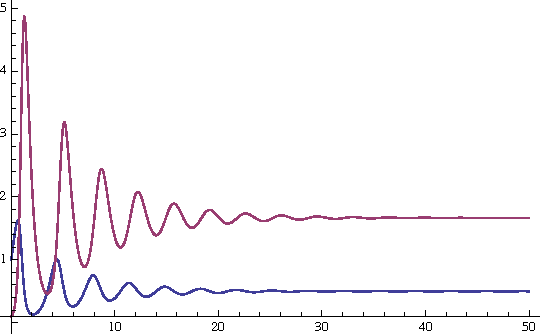
\includegraphics[width=10cm]{images/2_1_7d.pdf}
    \end{center}
\end{enumerate}
\subsection{2.1, Problem 10}%
We would add an extra $-\alpha F$ term to $\diff{F}{t}$ to account for the effect of hunting predators.
\subsection{2.1, Problem 14}%
If the prey move out at a rate proportional to the predators, we add an extra $-\beta F$ term to $\diff{R}{t}$ to account for the effect.
\subsection{2.2, Problem 7}%
\begin{enumerate}[(a)]
  \item We have
    \begin{align*}
      \diff{y}{t} &= v\\
      \diff{v}{t} &= y,
    \end{align*}
    so the vector field associated with this first order system is
    \begin{align*}
      \begin{pmatrix}\diff{y}{t}\\\diff{v}{t}\end{pmatrix} &= \begin{pmatrix}v(t)\\y(t)\end{pmatrix}.
    \end{align*}
  \item \hfill
    \begin{center}
      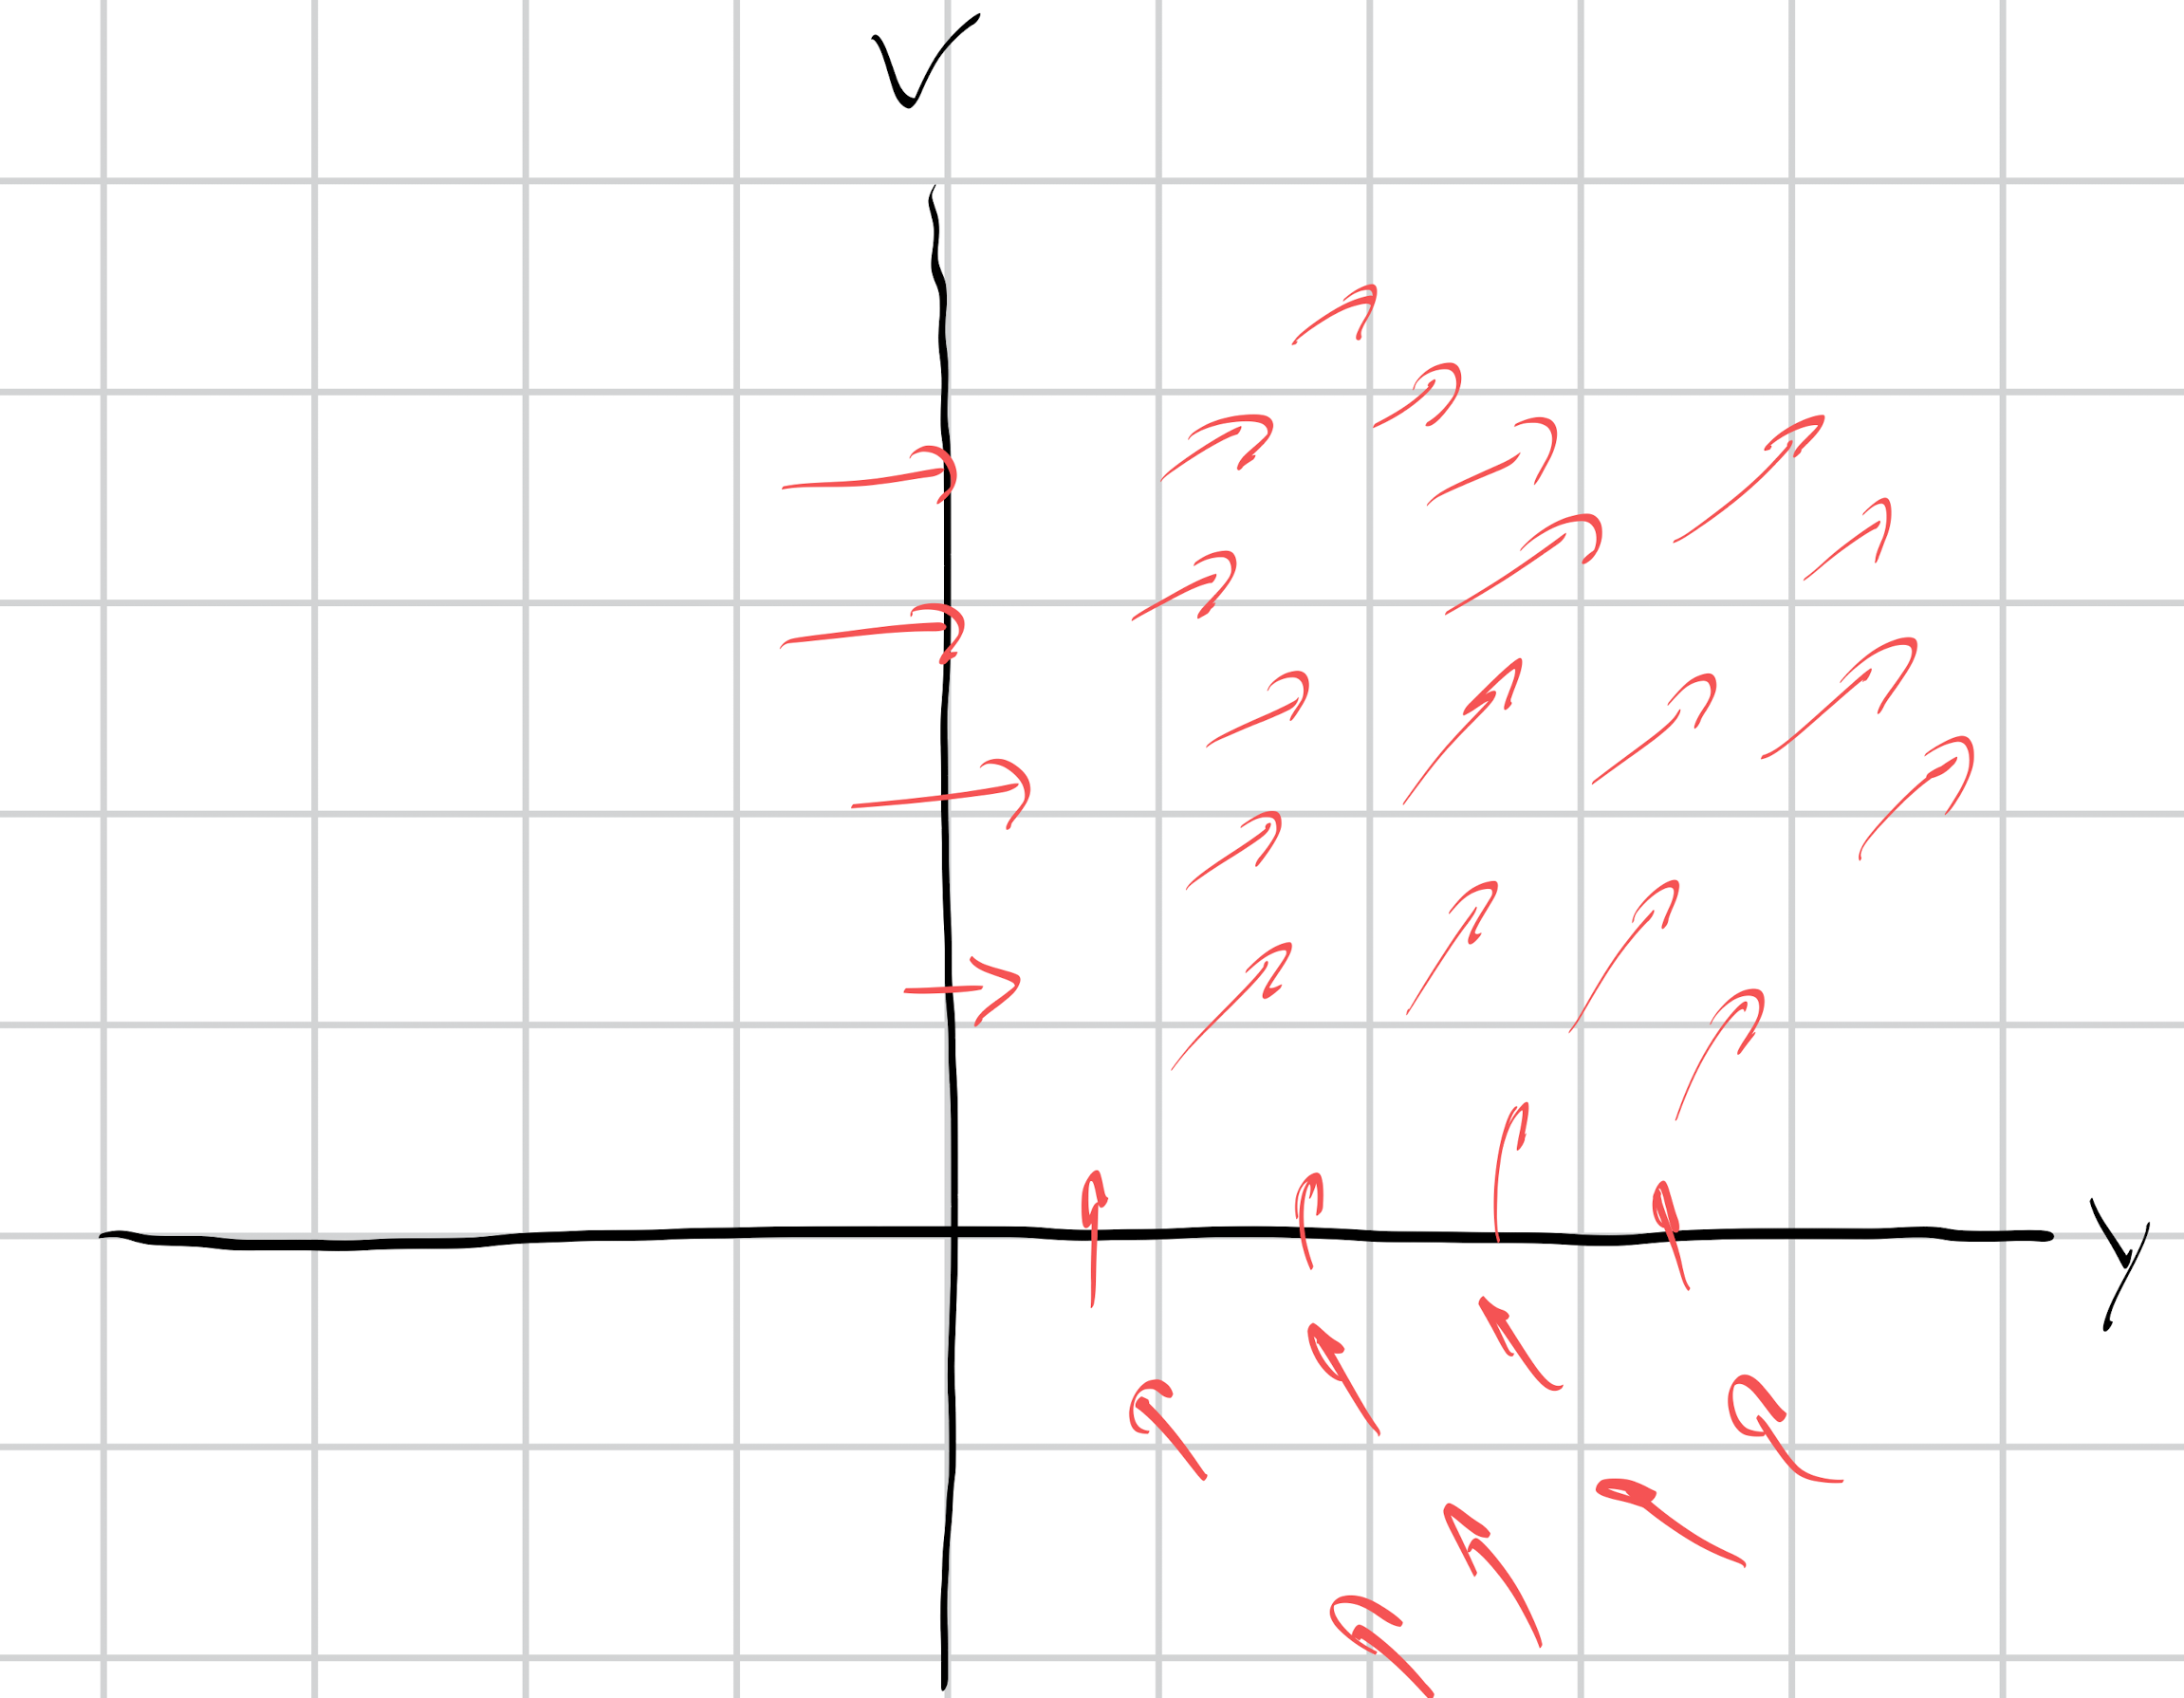
\includegraphics[width=10cm]{images/2_2_7b.png}
    \end{center}
  \item Using Mathematica:
    \begin{center}
      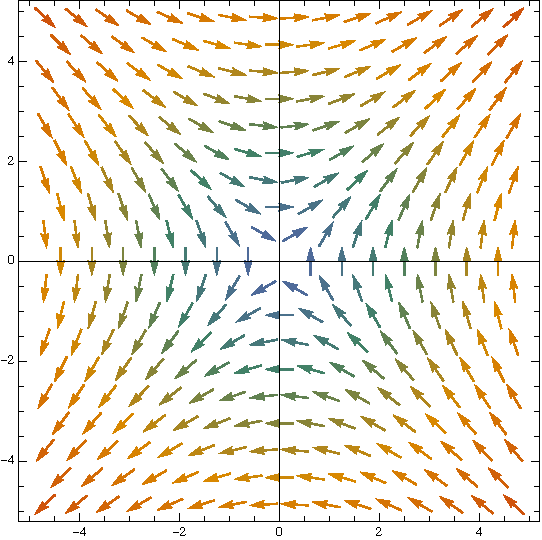
\includegraphics[width=10cm]{images/2_2_7c.pdf}
    \end{center}
  \item \hfill
    \begin{center}
      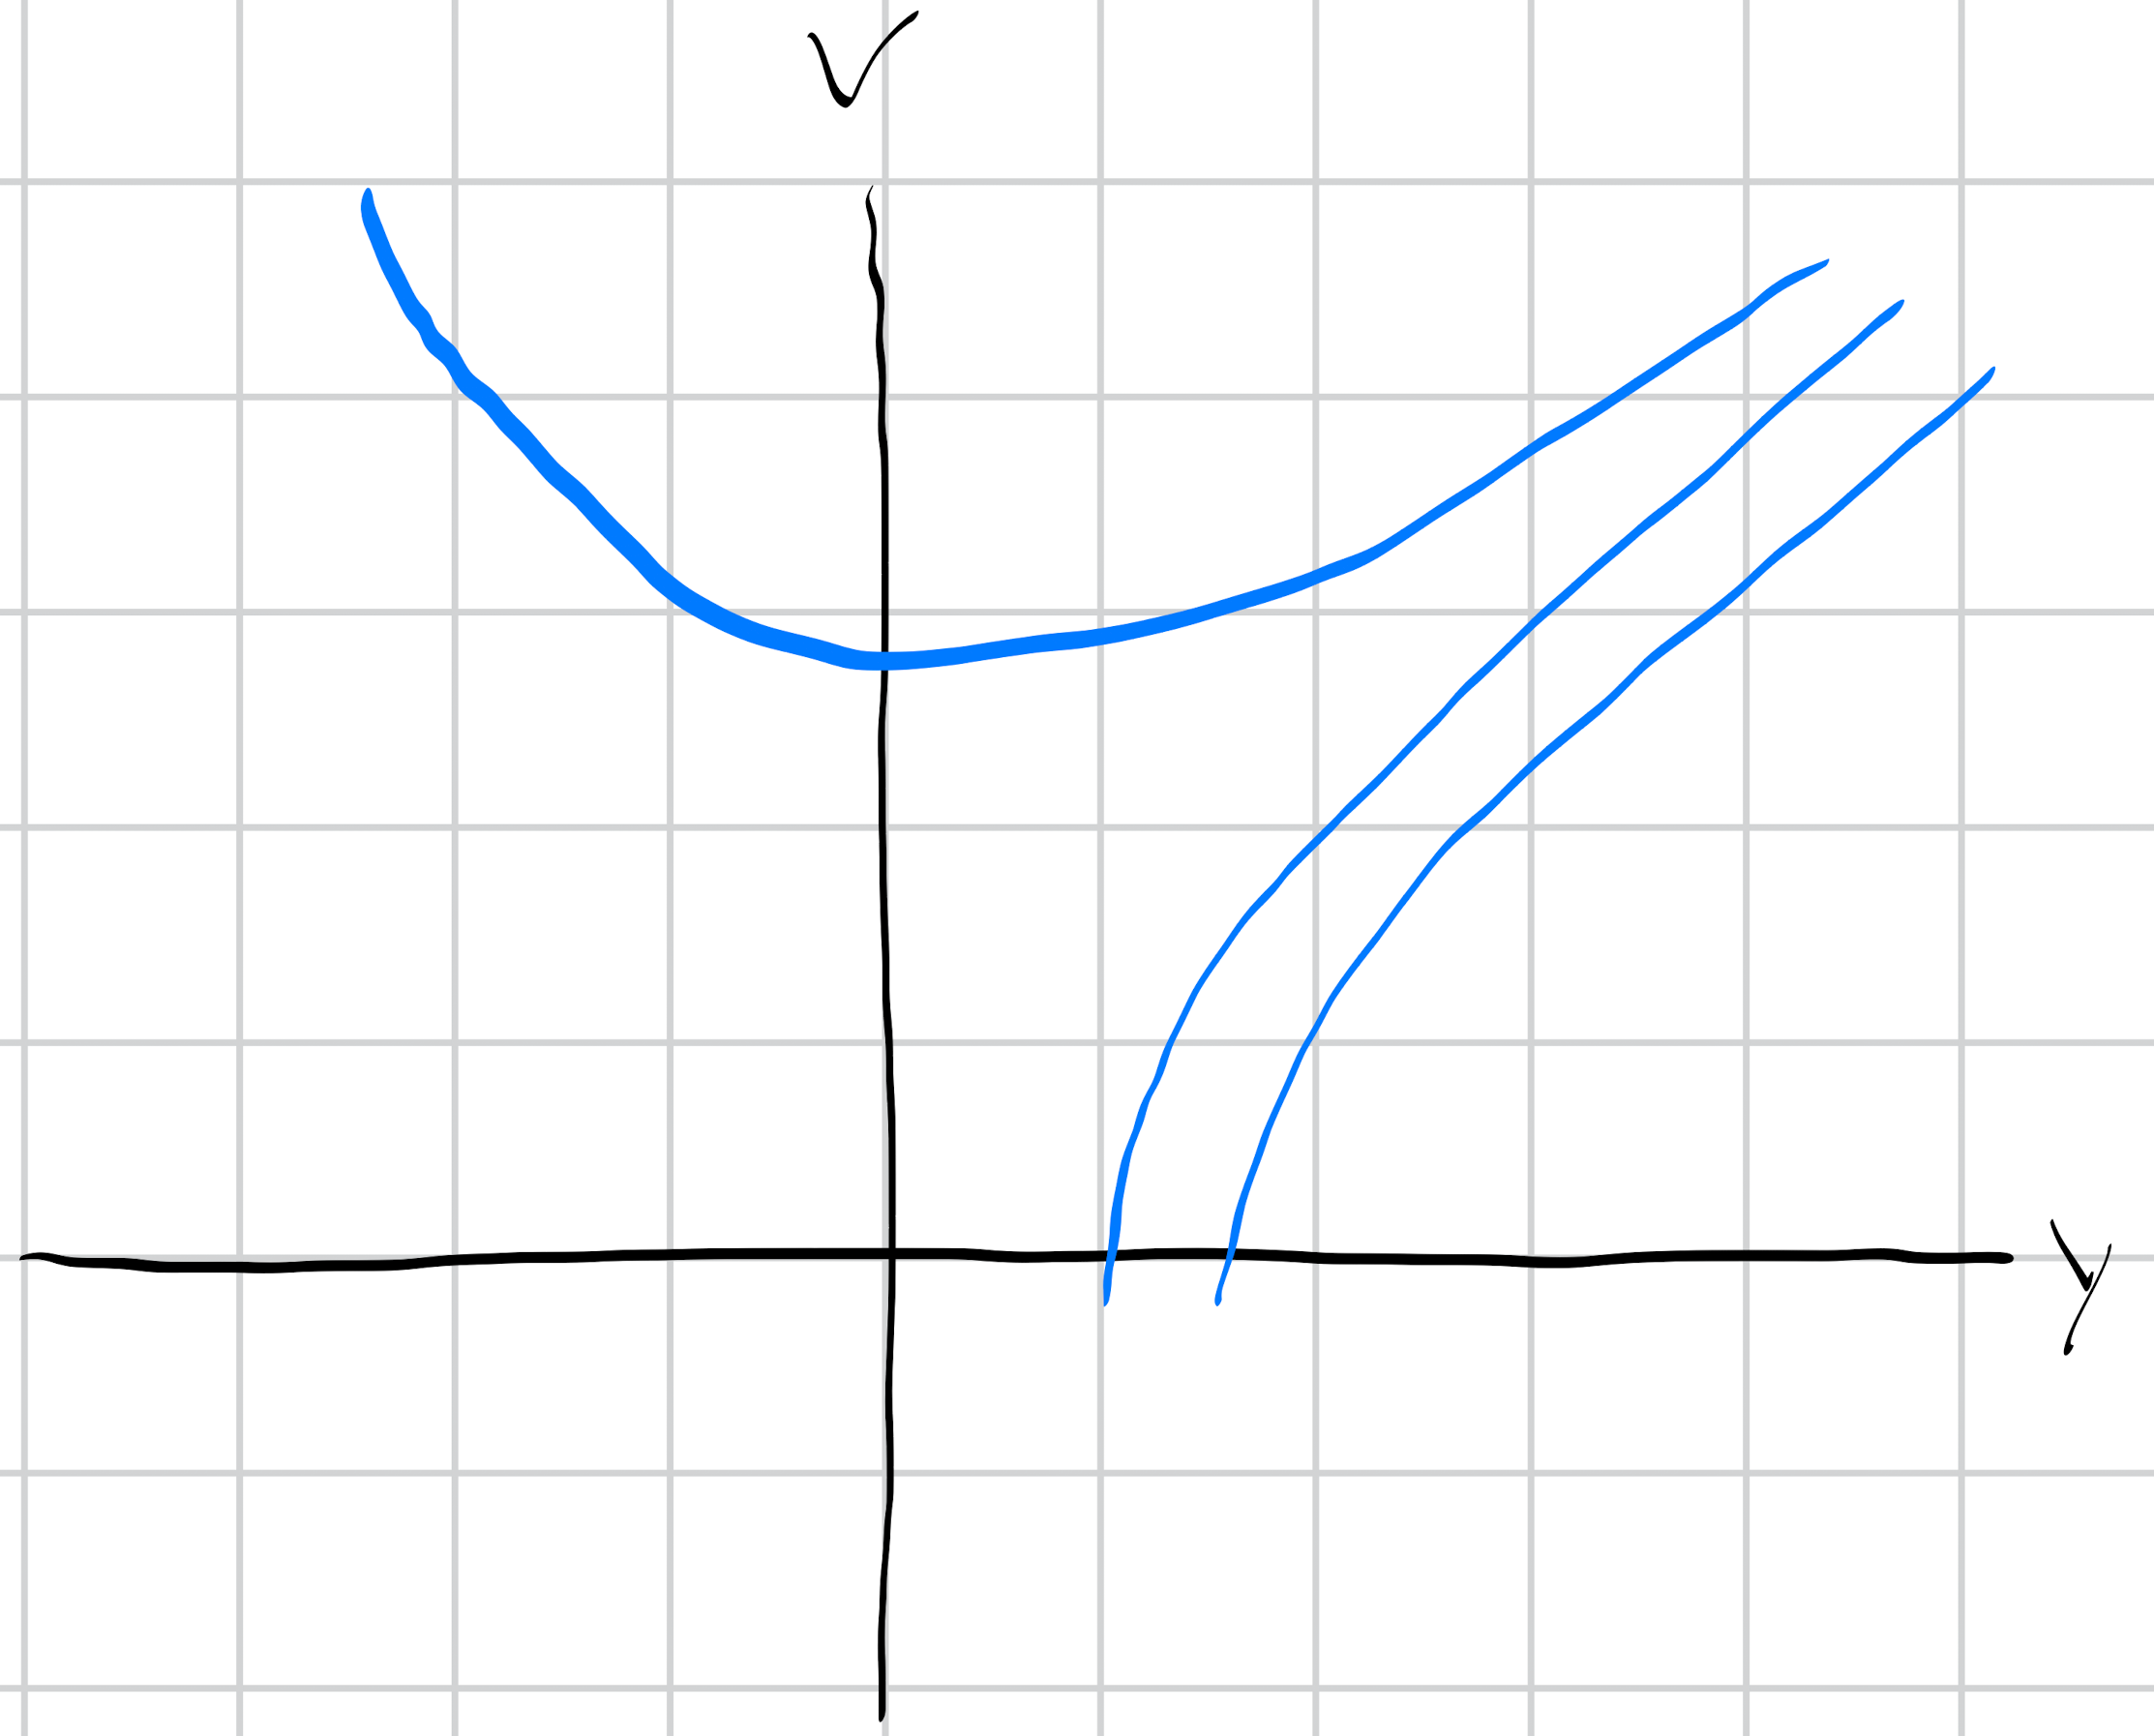
\includegraphics[width=10cm]{images/2_2_7d.png}
    \end{center}
  \item As $t$ goes to infinity, the solutions approach a ``blow up'' case.
\end{enumerate}
\subsection{2.2, Problem 8}%
\begin{enumerate}[(a)]
  \item We have
    \begin{align*}
      \begin{pmatrix}\diff{y}{t} \\ \diff{v}{t}\end{pmatrix} &= \begin{pmatrix}v(t)\\-2y(t)\end{pmatrix}
    \end{align*}
  \item \hfill
    \begin{center}
      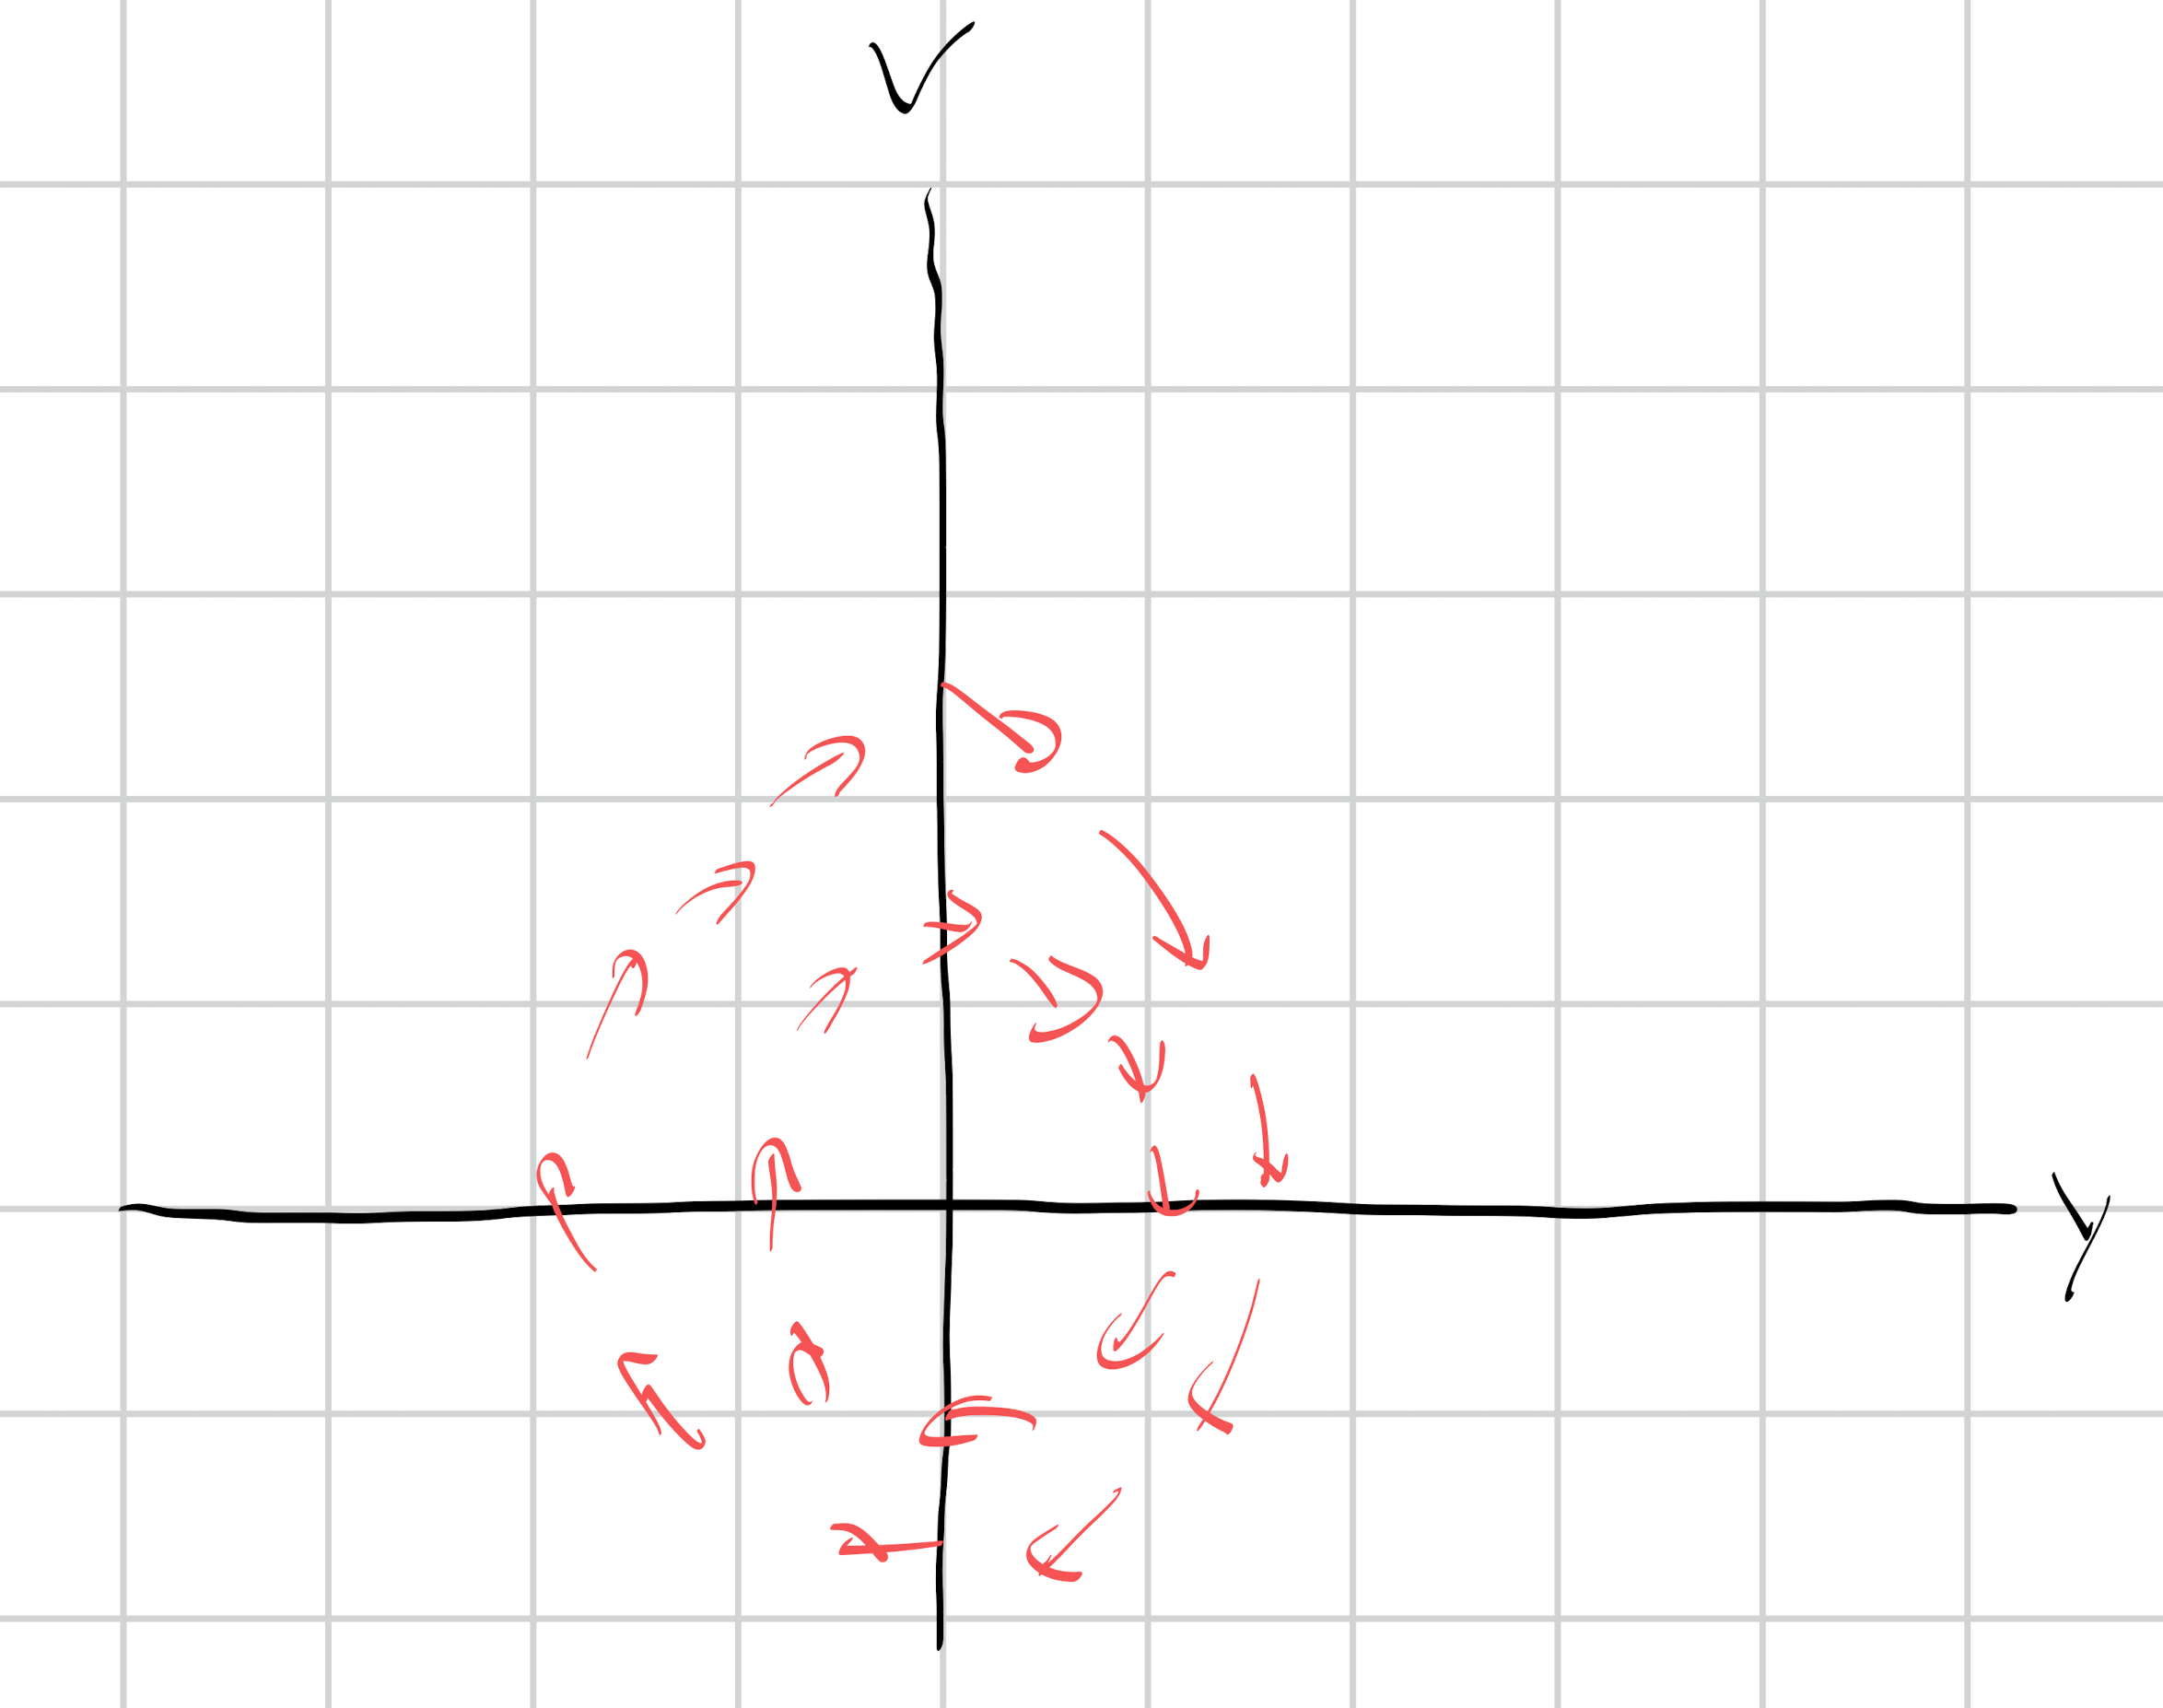
\includegraphics[width=10cm]{images/2_2_8b.png}
    \end{center}
  \item \hfill
    \begin{center}
      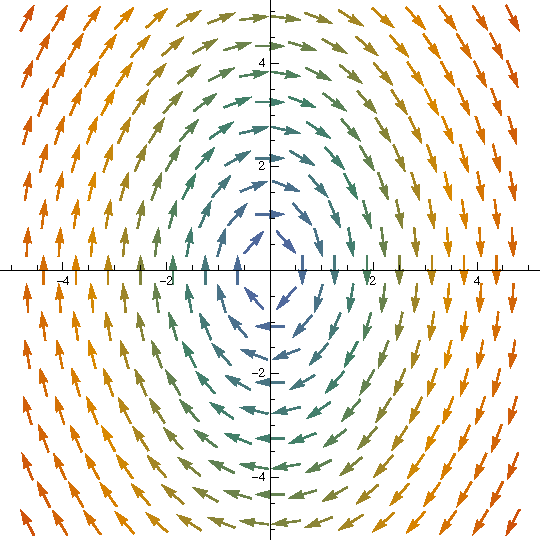
\includegraphics[width=10cm]{images/2_2_8c.pdf}
    \end{center}
  \item 
\end{enumerate}
\subsection{2.2, Problem 11}%
\begin{enumerate}[(a)]
  \item Since the $x$ components are $0$ at $x=\pm 1$, the two options are either (ii) or (vii). Since the slopes are negative for $x > 1$ and $y > 0$, it is the case that this slope field is (vii).
  \item This slope field corresponds to (viii), as the slope fields point to the origin for $y=x$.
  \item This slope field corresponds to system (iv), as it necessarily shoots away from the origin.
  \item This slope field corresponds to equation (vi), as for $x > 1$ and $y > 0$, the slopes are negative.
\end{enumerate}
\subsection{2.2, Problem 21}%
\begin{center}
  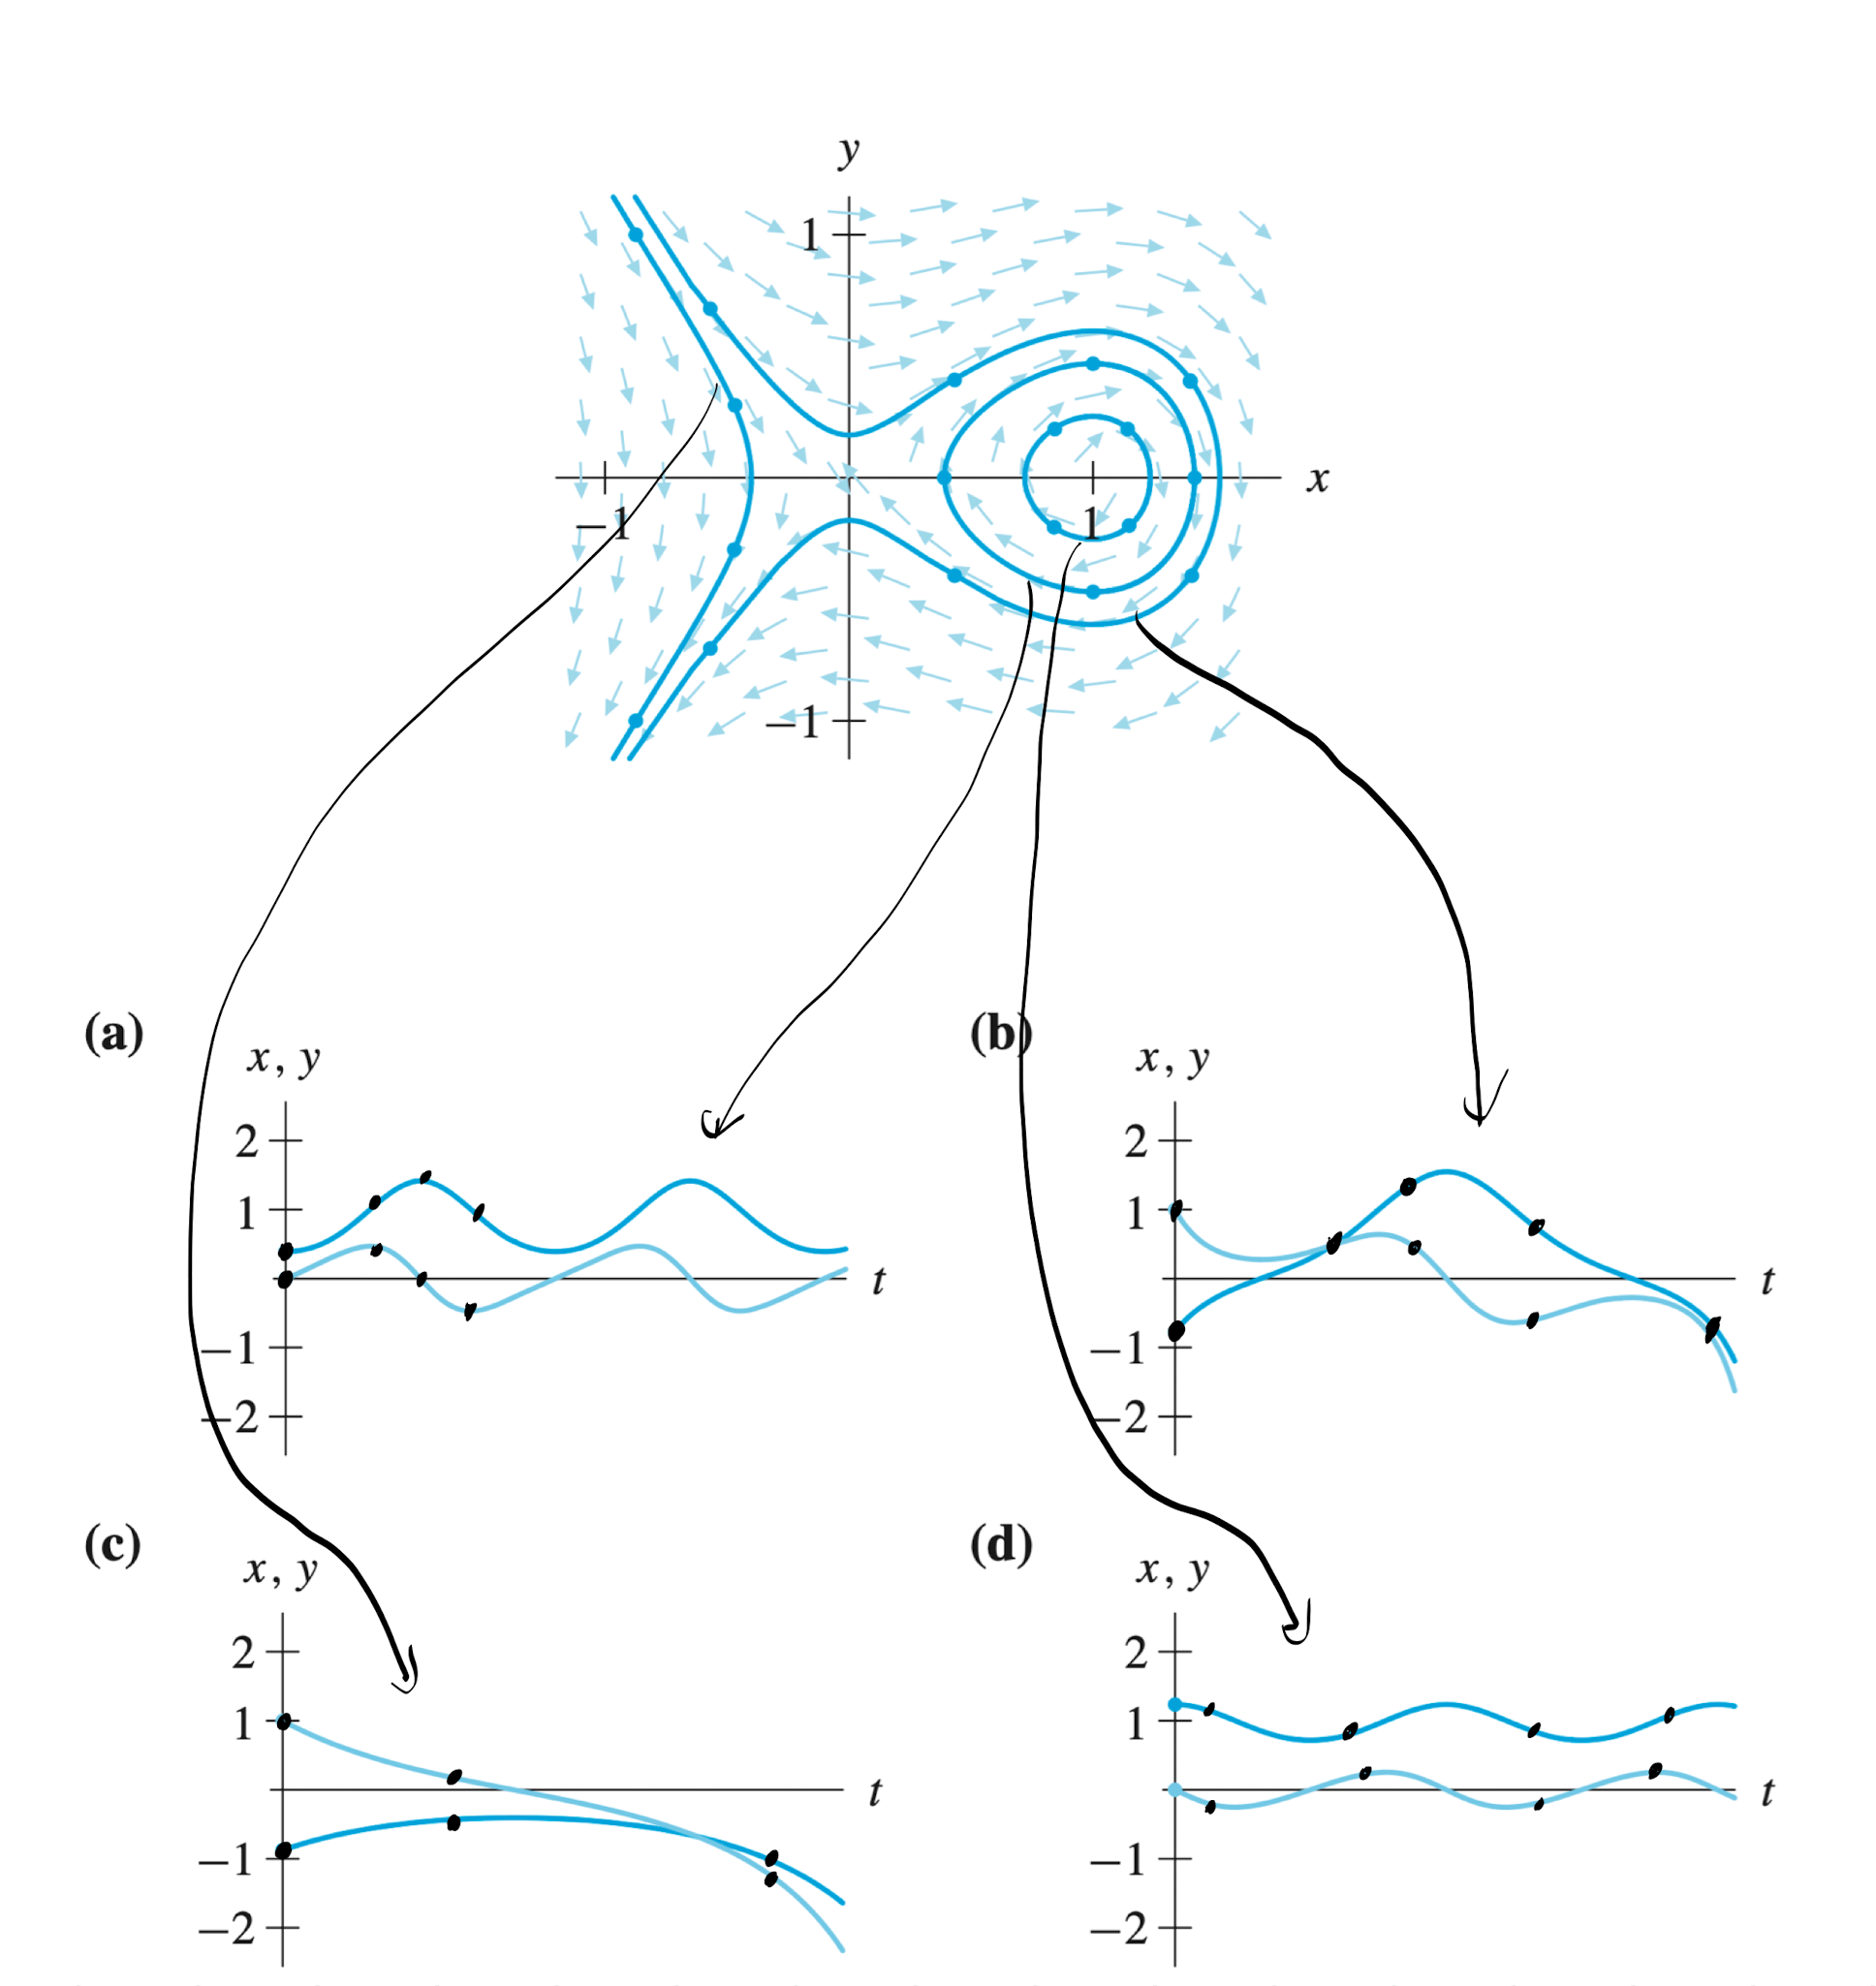
\includegraphics[width=10cm]{images/2_2_21.png}
\end{center}
\subsection{2.2, Problem 24}%
\begin{center}
  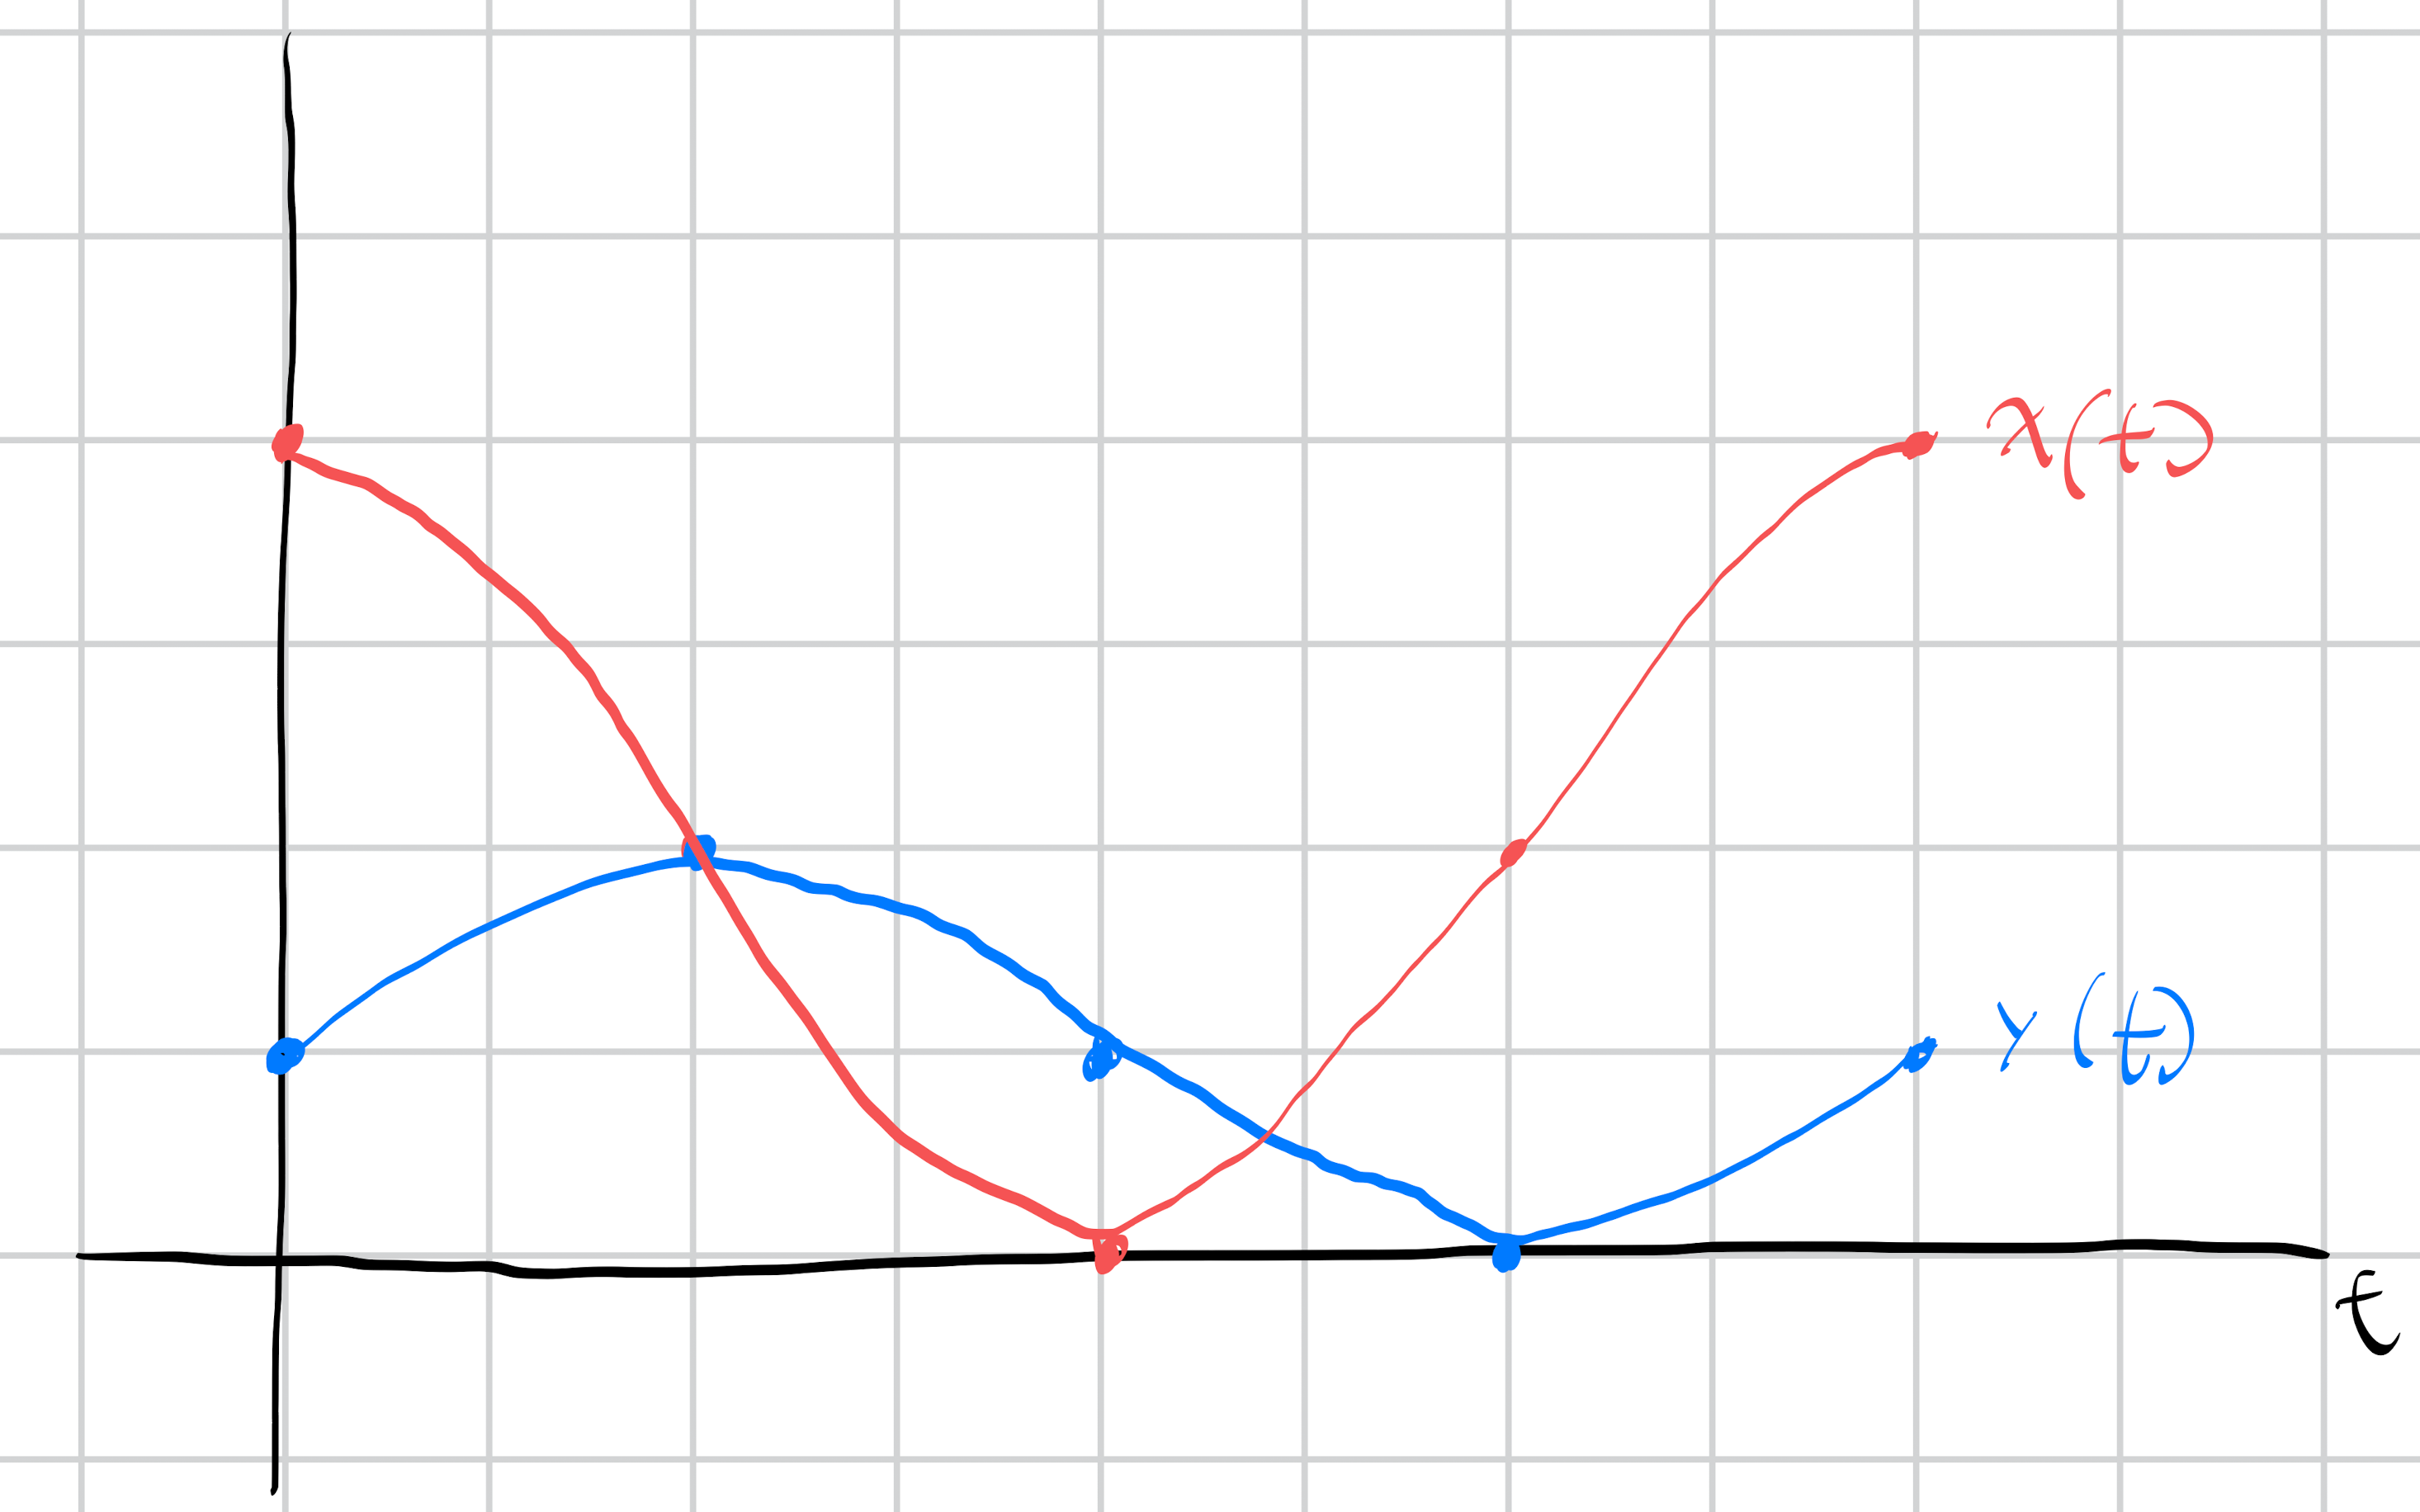
\includegraphics[width=10cm]{images/2_2_24.png}
\end{center}
\section{Part 2}%
\subsection{2.4, Problem 2}%
\begin{align*}
  \diff{x}{t} &= \diff{}{t}\left(3e^{2t} + e^{t}\right)\\
              &= 6e^{2t} + e^{t}\\
              &\neq 2\left(3e^{2t} + e^{t}\right) + 2\left(-e^{t} + e^{4t}\right).
\end{align*}
\subsection{2.4, Problem 5}%
The solution for $\diff{y}{t} = -y$ is of the form $y_0e^{-t}$, which this proposed solution does not have.
\subsection{2.4, Problem 7}%
Solving for $y$, we get $y(t) = k_2e^{-t}$. Substituting back in to the first equation, we have
\begin{align*}
  \diff{x}{t} &= 2x + k_2e^{-t}\\
  \diff{x}{t} - 2x &= k_2e^{-t}\\
  e^{-2t}\diff{x}{t} - 2xe^{-2t} &= k_2e^{-3t}\\
  \diff{}{t}\left(xe^{-2t}\right) &= k_2e^{-3t}\\
  xe^{-2t} &= -3k_2e^{-3t} + C\\
  x &= -3k_2e^{-3t} + k_1e^{2t}.
\end{align*}
Thus, the solution is
\begin{align*}
  \vec{Y}(t) &= \begin{pmatrix}-3k_2e^{-t} + k_1e^{2t}\\k_2e^{-t}\end{pmatrix}.
\end{align*}
\subsection{2.4, Problem 8}%
\begin{enumerate}[(a)]
  \item If we select $k_2 = 3$, then $-3k_2e^{-t} = -9e^{-t}$, which cannot equal $e^{-t}$.
  \item There is no $x$ dependence in the expression $\diff{y}{t}$.
\end{enumerate}
\subsection{2.4, Problem 9}%
\begin{enumerate}[(a)]
  \item If $y(0) = 0$, then $k_2 = 0$, meaning $k_1 = 1$. Thus, we get
    \begin{align*}
      \vec{Y}(t) &= \begin{pmatrix}e^{2t}\\0\end{pmatrix}.
    \end{align*}
  \item \hfill
    \begin{center}
      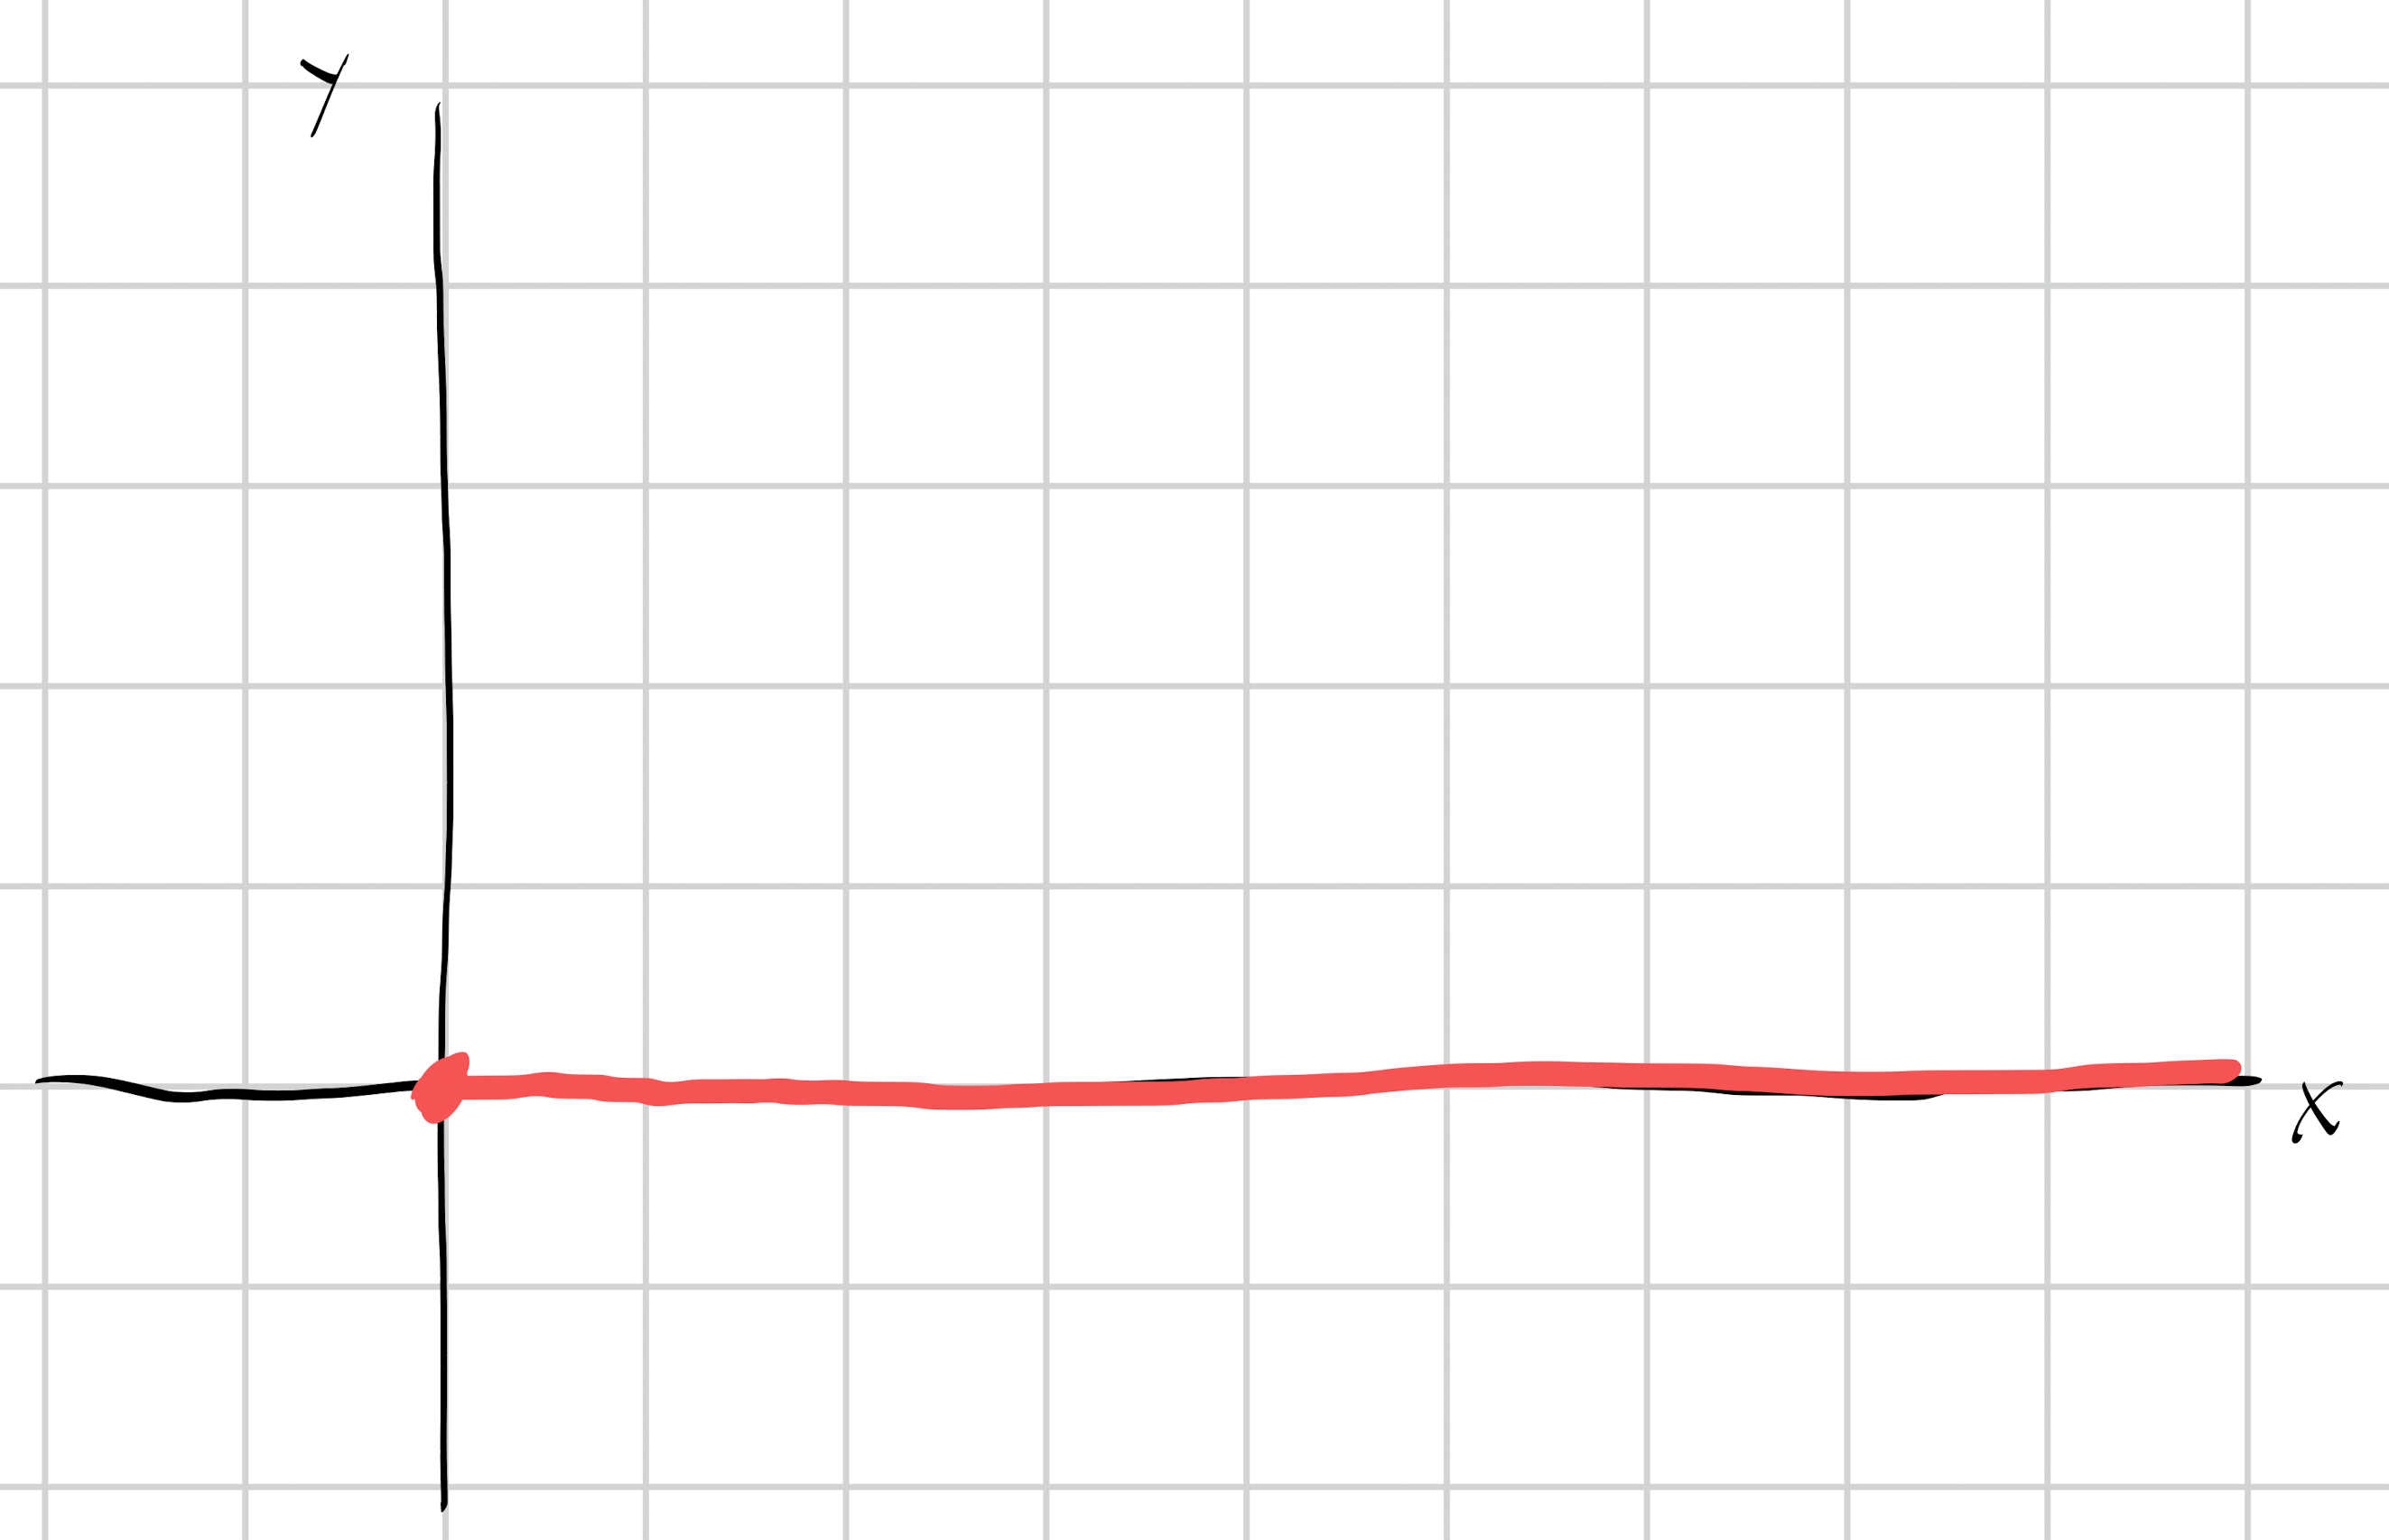
\includegraphics[width=10cm]{images/2_4_9b.png}
    \end{center}
  \item \hfill
    \begin{center}
      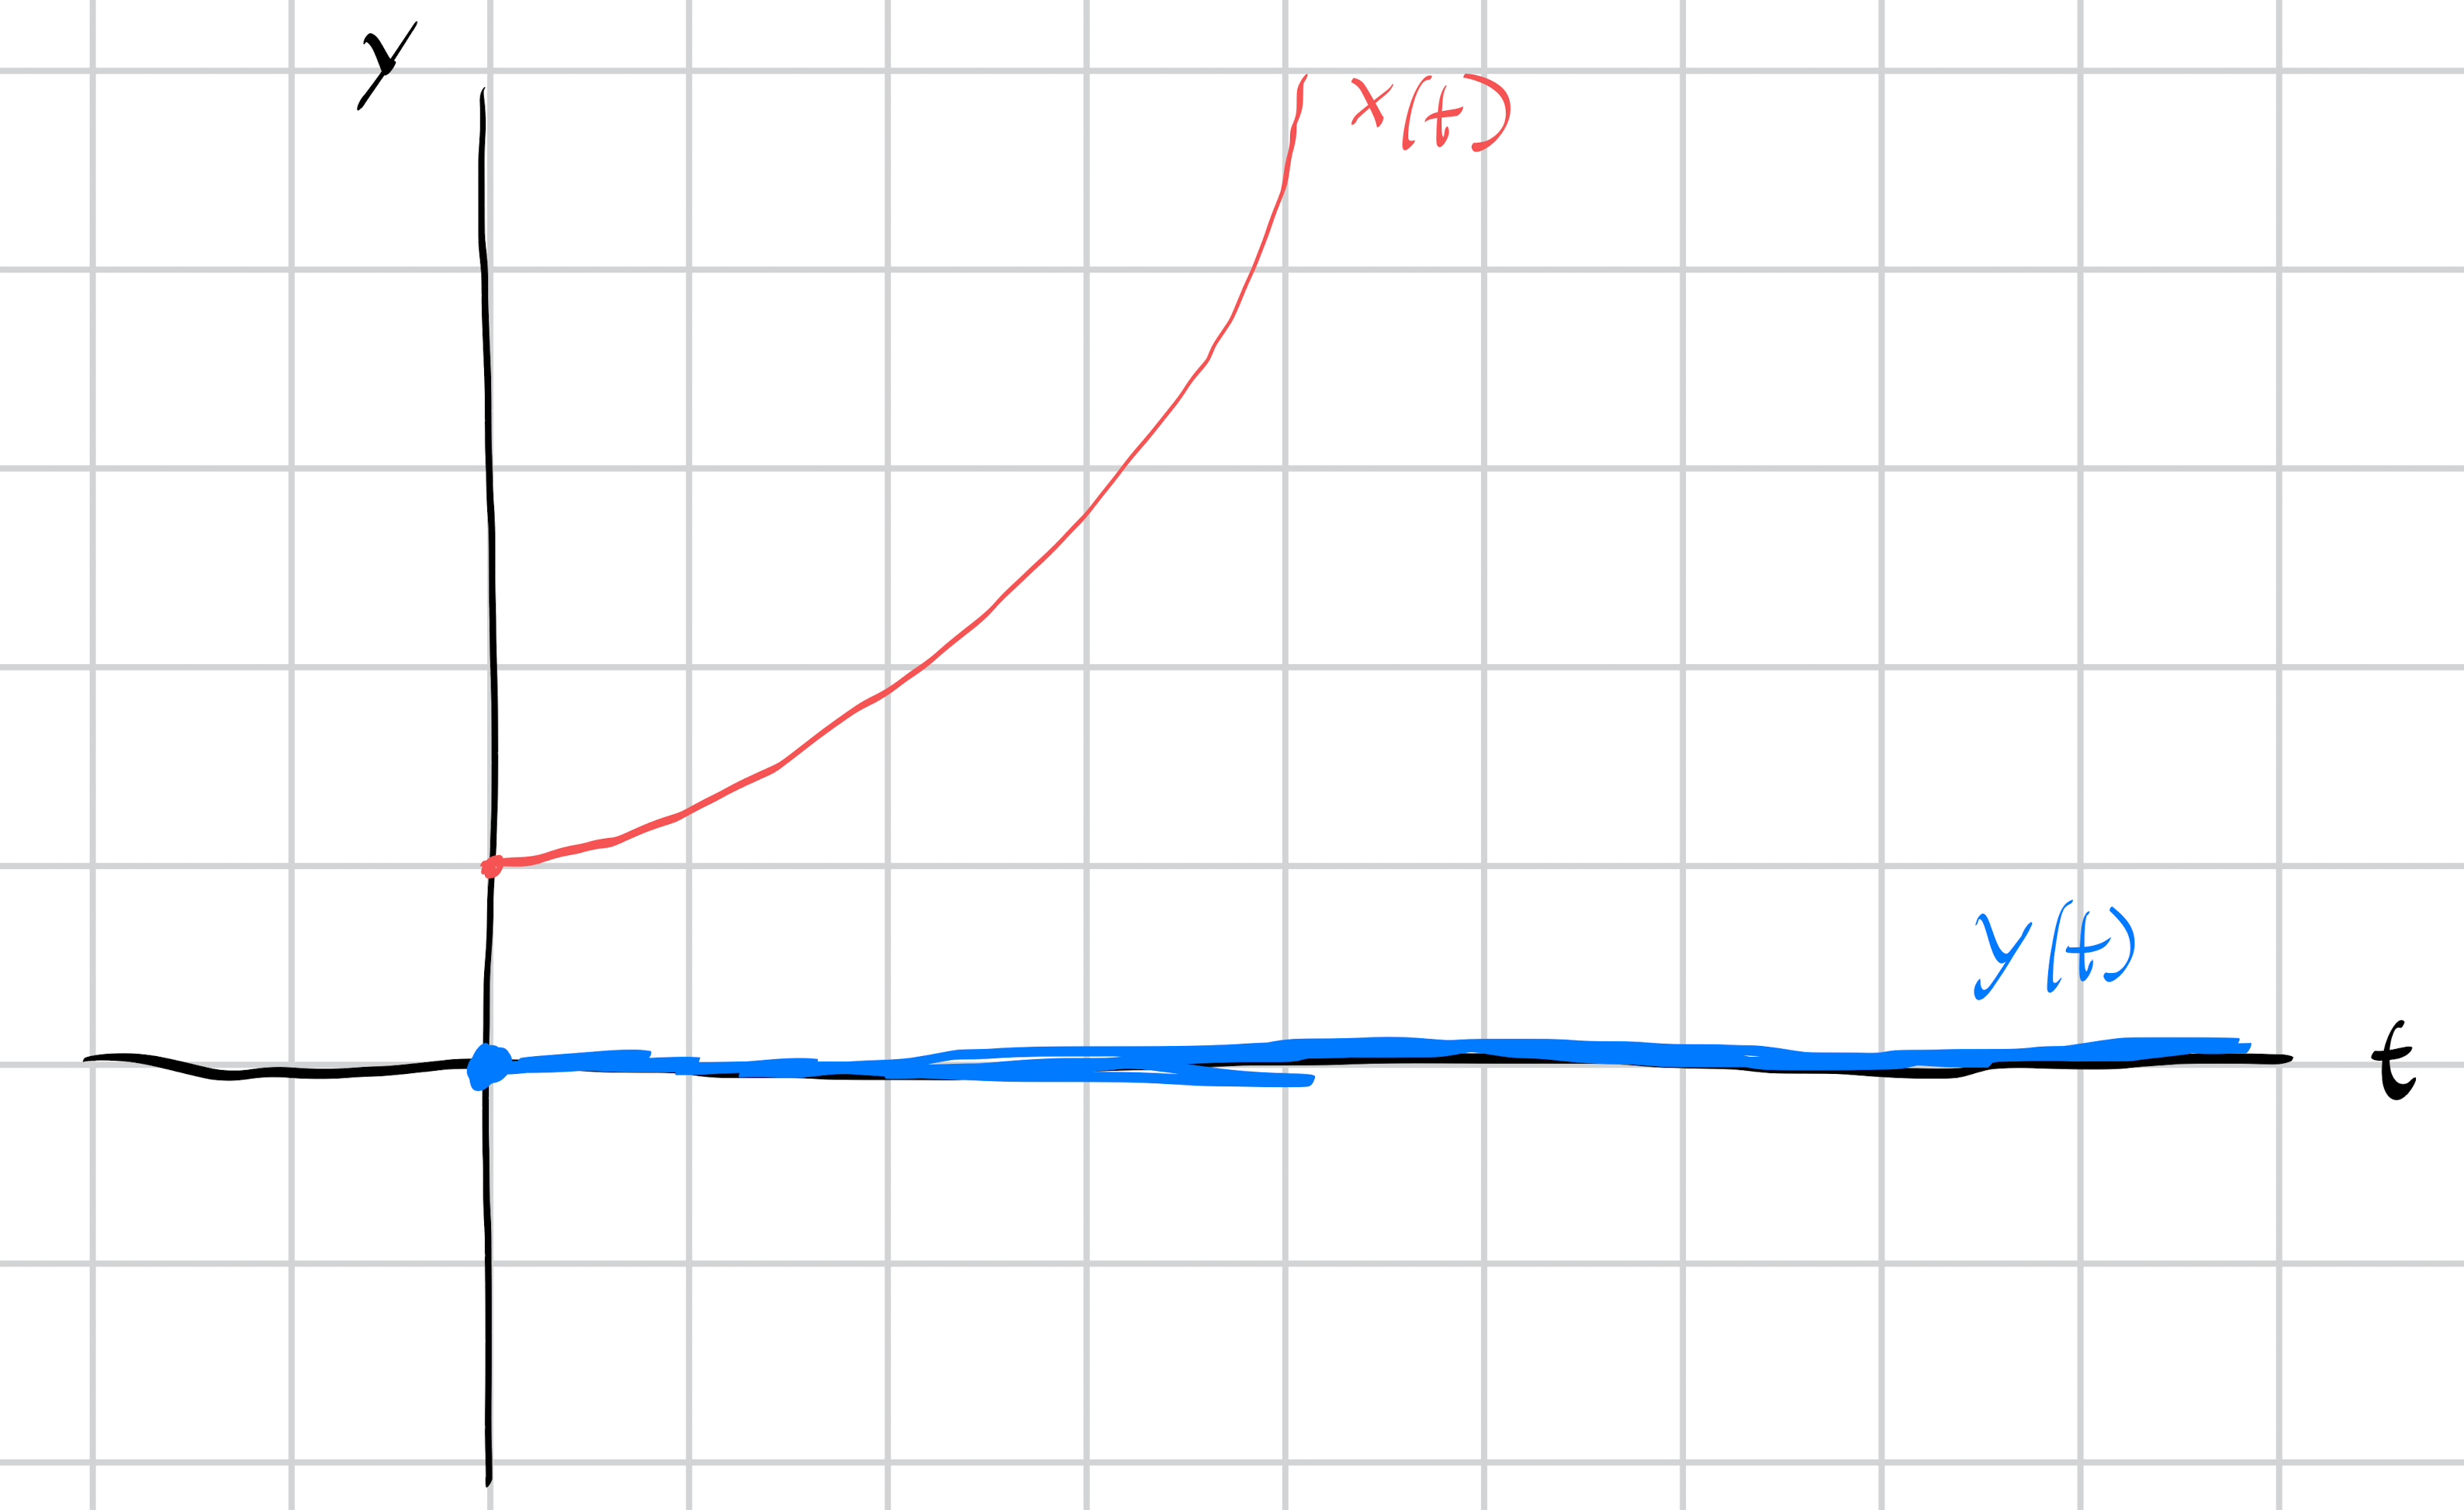
\includegraphics[width=10cm]{images/2_4_9c.png}
    \end{center}
\end{enumerate}
\subsection{2.4, Problem 13}%
\begin{enumerate}[(a)]
  \item We solve $\diff{y}{t} = -3y$, yielding $y(t) = k_2e^{-3t}$. Substituting into $\diff{x}{t}$, we get
    \begin{align*}
      \diff{x}{t} &= 2x - 8k_2e^{-6t}\\
      \diff{x}{t} - 2x &= -8k_2e^{-6t}\\
      e^{-2t}\diff{x}{t} - 2xe^{-2t} &= -8k2e^{-8t}\\
      xe^{-2t} &= 64k_2e^{-8t} + k_1\\
      x &= 64k_2e^{-8t} + k_1e^{2t}.
    \end{align*}
  \item We have $\diff{y}{t} = 0$ only if $k_2 = 0$, meaning $\diff{x}{t} = 0$ only if $\diff{x}{t}= 2x = 0$, so the only equilibrium point is at $(0,0)$.
  \item Substituting into the expression for $y(t)$, we get $y(t) = e^{-3t}$. Substituting for $x$, we get
    \begin{align*}
      0 &= 64 + k_1e^{2t}\\
      k_1 &= -64,
    \end{align*}
    meaning the solution that satisfies this initial condition is
    \begin{align*}
      \begin{pmatrix}\diff{x}{t}\\\diff{y}{t}\end{pmatrix} &= \begin{pmatrix}64e^{-8t} - 64e^{2t}\\e^{-3t}\end{pmatrix}.
    \end{align*}
  \item I can't solve using Mathematica.
\end{enumerate}
\subsection{2.5, Problem 2}%
\begin{enumerate}[(a)]
  \item Since the system is fully decoupled, and $e^{2t}$ is a system for $\diff{x}{t} = 2x$, while $3e^{t}$ is a solution to $\diff{y}{t} = y$, this is a solution.
  \item At $t=2$ the approximate solution is $(16,15.19)$, while the exact solution is $(54.60,22.17)$.\newline

    At $t = 4$, the approximate solution is $(256,76.88)$, while the exact solution is $\left(2980,163.8\right)$.\newline

    At $t=6$, the approximate solution is $\left(4096,389.24\right)$, while the exact solution is $\left(162755,1210.3\right)$.
  \item At $t=2$, the approximate solution is $\left(38.33,20.18\right)$.\newline

    At $t=4$, the approximate solution is $\left(1470,136\right)$.\newline

    At $t=6$ the approximate solution is $\left(56347,913.44\right)$.
  \item The approximations are generally on the basis of slope, and so diverge as the exponential function grows much faster than any linear approximation.
\end{enumerate}
\subsection{2.5, Problem 3}%
\begin{enumerate}[(a)]
  \item The estimated output from Euler's method has a final result of $\left(0.09375,-0.09375\right)$.
  \item \hfill
    \begin{center}
      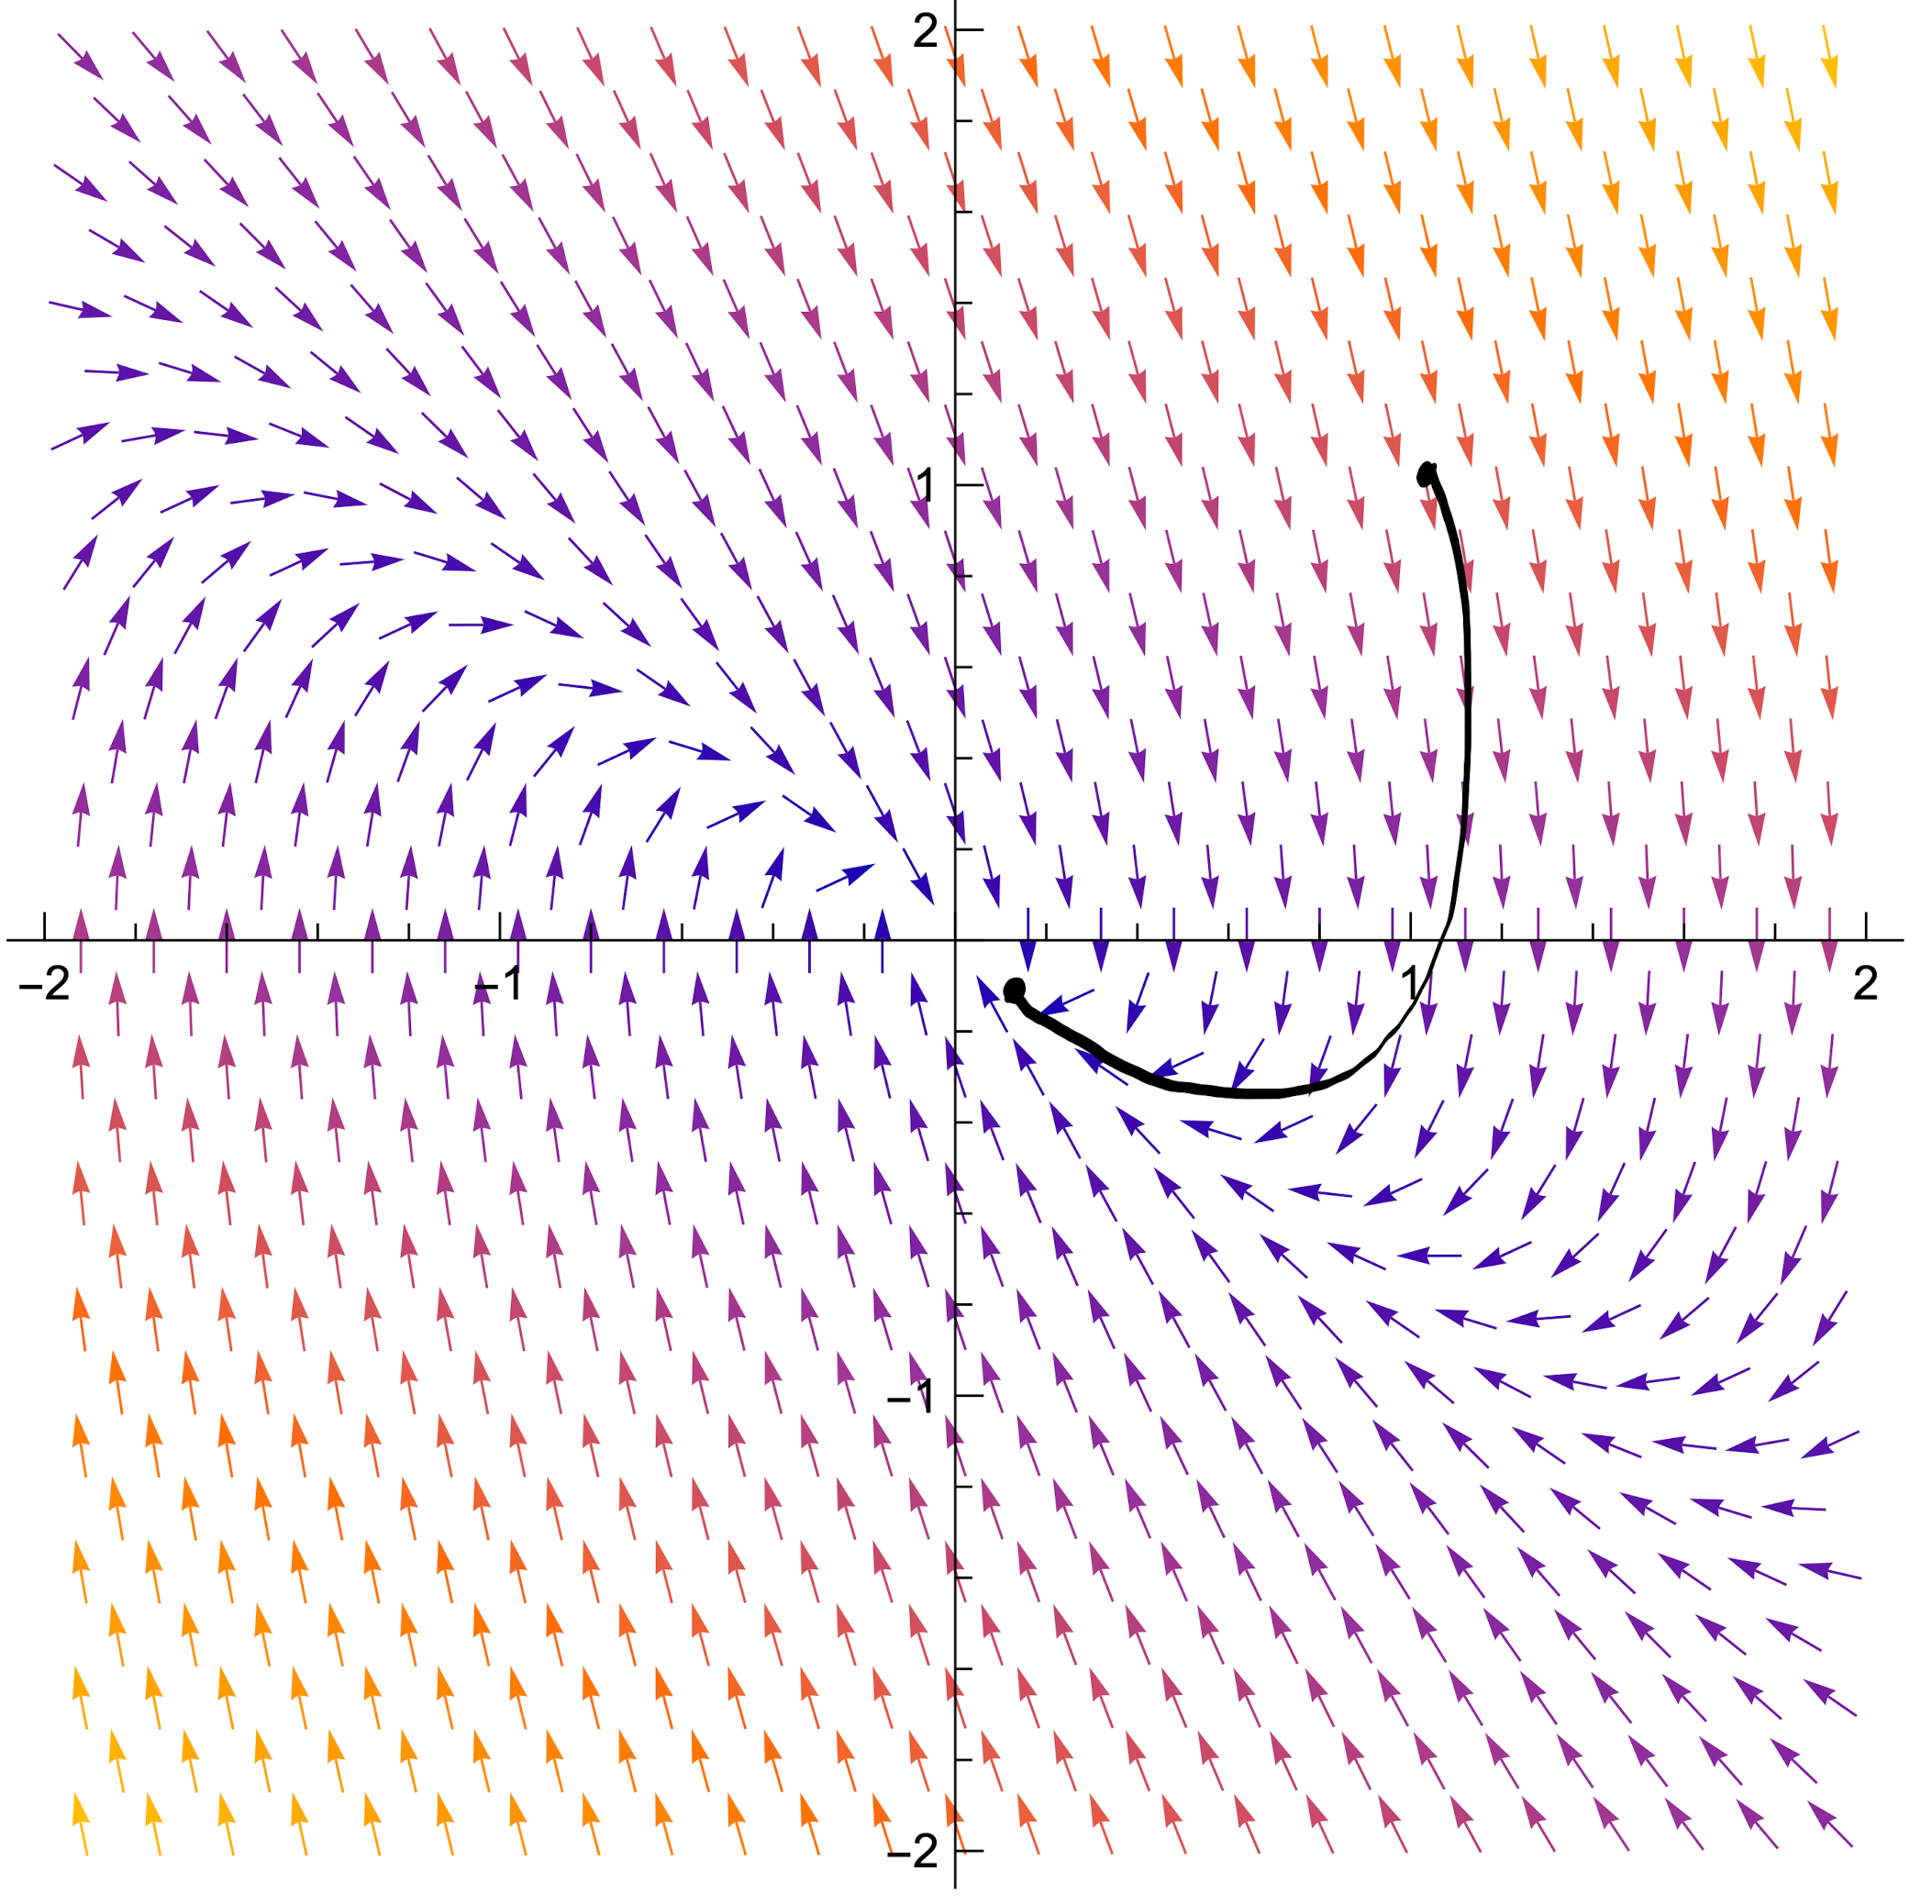
\includegraphics[width=10cm]{images/2_5_3b.png}
    \end{center}
  \item \hfill
    \begin{center}
      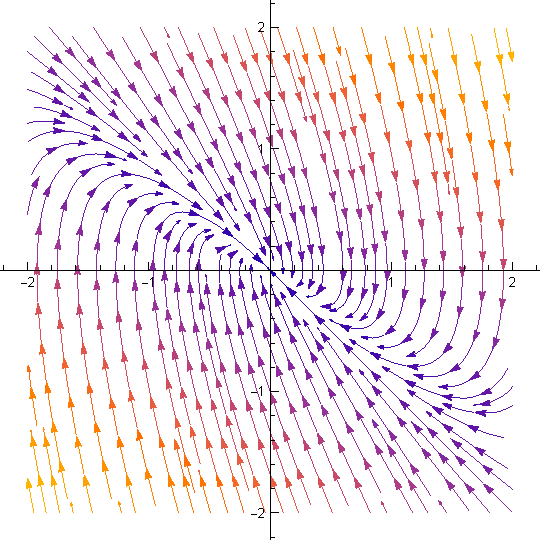
\includegraphics[width=10cm]{images/2_5_3c.pdf}
    \end{center}
\end{enumerate}
\end{document}
